\documentclass[a4paper,11pt]{article}
\usepackage[utf8x]{inputenc}
% \usepackage[latin1]{inputenc}
\usepackage[brazil]{babel}
\usepackage[pdftex]{color,graphicx}
\usepackage[a4paper,left=2.2cm,right=2.3cm,top=2.5cm,bottom=2.5cm]{geometry}
\usepackage{subfig}
\usepackage{picinpar}
\usepackage{multicol}
\usepackage{bm}
% \usepackage{program}
\usepackage{varwidth}
\usepackage{parskip}
\usepackage{algorithm}
\usepackage{algpseudocode}
\usepackage{hyperref}
\usepackage{natbib}
\usepackage{url}
\usepackage{pbox}
\usepackage{footnote}




\title{ Classificando spams em uma pequena base \\ de dados de mensagens SMS}

\author{Renzo A. Viloche Morales \\ \texttt{renvmorales@gmail.com}}


\begin{document}

\DeclareGraphicsExtensions{.jpg,.pdf,.mps,.png}
\maketitle

\section{Introdução}

Mineração de texto é comumente usada com a finalidade de analisar e obter uma descrição geral em 
dados não-estruturados (por exemplo, um texto único, ou mensagens enviadas a partir de vários 
usuários). Este tipo de operação não é apenas importante para fins de uma análise exploratória, 
mas também necessário durante a etapa de pré-processamento que fornecerá dados de entrada para 
treinar um modelo (algoritmo) de classificação através de uma técnica de aprendizado de máquina. 

Neste trabalho, uma pequena base de dados de 5.574 mensagens SMS contendo spams (mensagens 
consideradas fora do interesse do destinatário) é analisada brevemente e convertida numericamente 
usando a técnica de \textit{tf-idf}. Uma vez concluído o processamento, a base de dados é dividida 
em duas partes: uma para ``teste'' e outra para ``treinamento''. O objetivo aqui é avaliar 
rapidamente, através de validação cruzada com $k$-pastas, a capacidade de classificação para 
quatro modelos de aprendizado: \textit{naïve-Bayes}, regressão logística, SVM (\textit{support 
vector machine}) e \textit{Multi-layer Perceptron}. As análises, validação de performance dos 
modelos são todos realizados usando a linguagem de código aberto Python, mais especificamente os 
módulos: \textit{numpy, pandas, scikit-learn, wordcloud, nltk, string}.


% Text mining is commonly used to provide some general description into unustructured data 
% (e.g, single text or multiple collected user messages). This operation is important not just for 
% exploratory data analysis purposes, but also when performing a preprocesing step required in order 
% to apply a machine learning technique such as a classification algorithm. Here a small dataset of 
% SMS messages is analyzed and prepared.





\section{Descrição da base de dados}

A base de dados contida no arquivo \texttt{SMS.csv} é composta por diversas mensagens comuns (4.827)
e spams (747) em inglês dispostos na forma de 5.574 linhas e 154 colunas. Os atributos (cada coluna) 
da base de dados são descritos a seguir:

\begin{itemize}
 \item 1 coluna contendo a mensagem original (\texttt{Full\_Text});
 \item 149 colunas com valores inteiros que indicam a frequência de uma determinada palavra na 
 mensagem (\texttt{got ... wan});
 \item 1 coluna contendo a quantidade de palavras frequentes na mensagem 
 (\texttt{Common\_Words\_Count});
 \item 1 coluna contendo a quantidade total de palavras da mensagem (\texttt{Word\_Count});
 \item 1 coluna contendo a data de recebimento da mensagem (\texttt{Date});
 \item 1 coluna que identifica se a mensagem é spam ou não (\texttt{IsSpam}).
\end{itemize}

Sempre que possível, a base de dados neste trabalho será referida como \texttt{SMS}.



\subsection{Análise exploratória}

Inicialmente foi realizado uma análise das palavras mais frequentes em toda a base. Para isto, 
as frequências totais de cada uma das 149 palavras mais comuns foram calculadas. O seguinte gráfico 
de barras na figura \ref{fig:barplot} exibe cada uma das frequência para palavras com frequência de 
no mínimo igual a 150.

\begin{figure}[htbp]
    \centering
    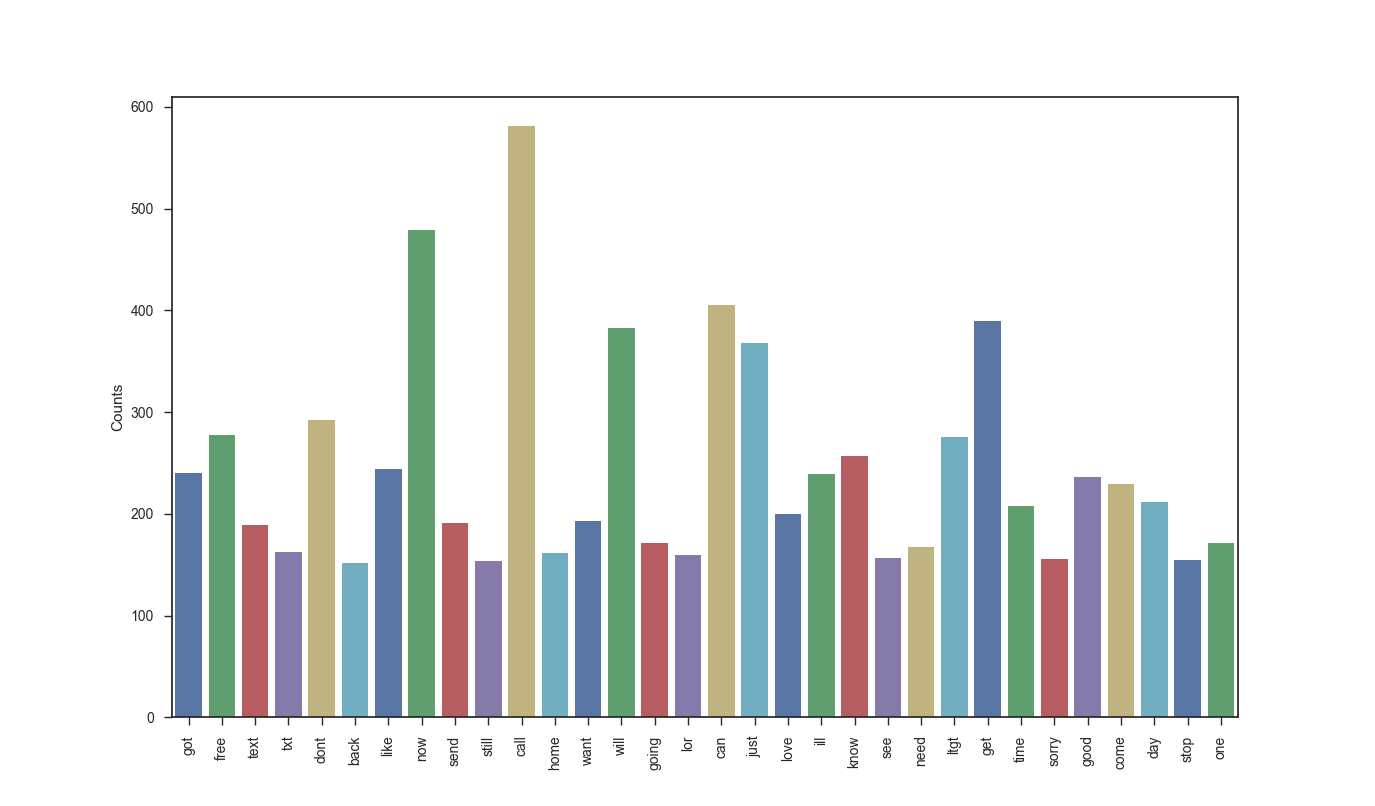
\includegraphics[width=\textwidth]{word_barplot.png}
    \caption[Figura simples]{Gráfico de barras com frequências de palavras mais comuns de 
    \texttt{SMS} superiores a 150.}
    \label{fig:barplot}
\end{figure}

O gráfico mostra 32 palavras com ocorrência superior ao mínimo estabelecido (para efeito de melhor
visualização). A lista completa destas palavras é: \texttt{got, free, text, txt, dont, back, 
like, now, send, still, call, home, want, will, going, lor, can, just, love, ill, know, see, need, 
ltgt, get, time, sorry, good, come, day, stop, one}.

Um outro recurso de mais fácil visualização é a nuvem de palavras. Nela, o tamanho de cada palavra 
é proporcional a sua frequência de ocorrência. Neste caso uma nuvem de palavras foi aplicada sobre 
o universo de palavras mais comuns. A figura \ref{fig:wordcloud} apresenta a nuvem com as 50 palavras 
de maior ocorrência. Através do recurso de nuvem fica muito mais fácil identificar, por exemplo,
que as palavras mais utilizadas foram: \texttt{call, can, now, will, get, just}.


\begin{figure}[htbp]
    \centering
    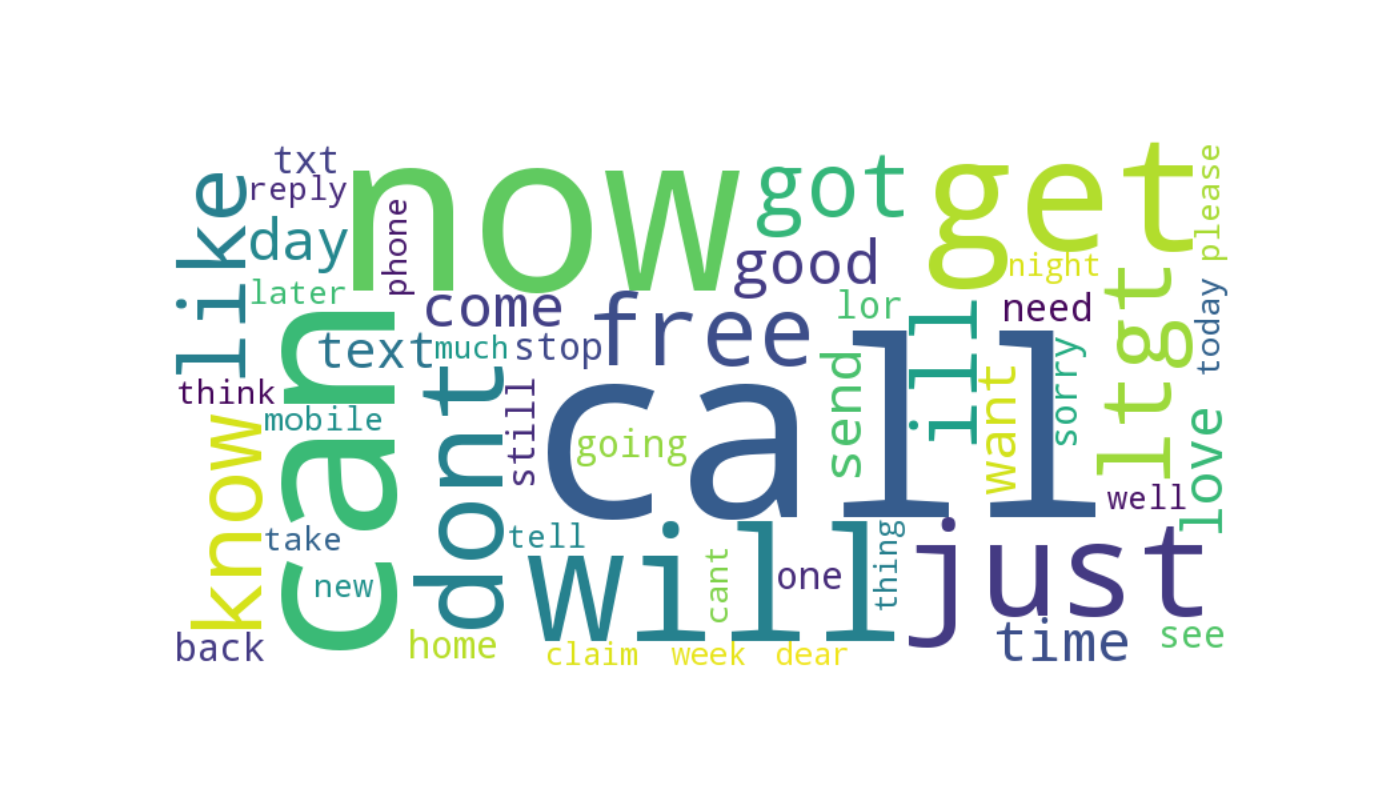
\includegraphics[width=\textwidth]{word_cloud.png}
    \caption[Figura simples]{Nuvem com as 50 palavras mais frequentes dentro de um universo de 
    palvras mais comuns de \texttt{SMS}.}
    \label{fig:wordcloud}
\end{figure}


\newpage
A seguir, foi feita uma análise da quantidade de mensagens normais e de spam por mês. O 
gráfico de barras na figura \ref{fig:monthly_spam} apresenta estas quantidades para os meses de Janeiro, Fevereiro 
e Março. É possível ver que o número de mensagens classificadas como ``spam'' é bem reduzido 
quando comparado ao número de mensagens comuns. O número de spams aparenta posuir mais 
homogeneidade e uma frequência superior a 200 vezes por mês.


\begin{figure}[htbp]
    \centering
    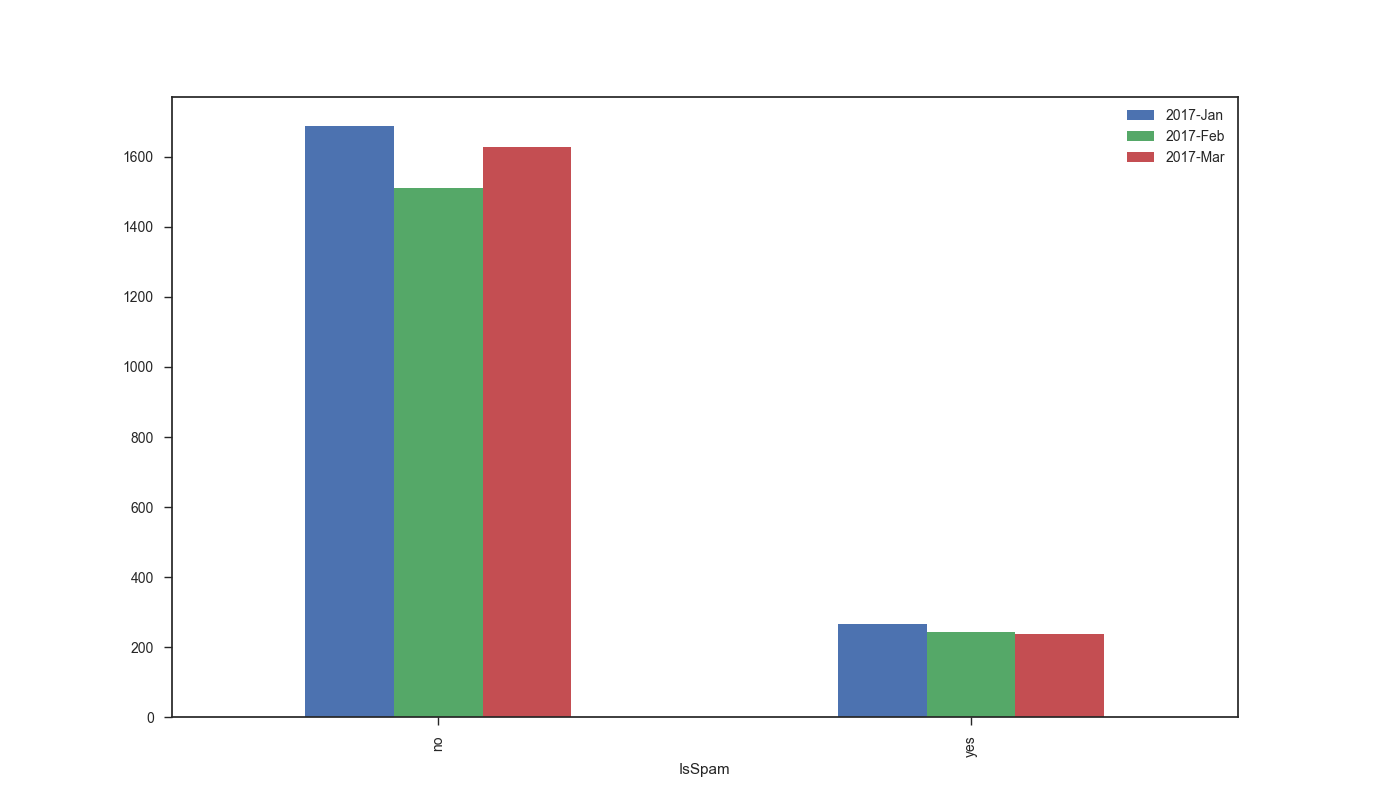
\includegraphics[width=\textwidth]{monthly_spam.png}
    \caption[Figura simples]{Número mensal de mensagens comuns vs. spams para \texttt{SMS}.}
    \label{fig:monthly_spam}
\end{figure}


Para o atributo \texttt{Word\_Count}, um número de estatísticas descritivas foram calculadas: 
max, min, média, mediana e desvio padrão. A tabela \ref{tab:stats} apresenta o cenário encontrado para
esta variável.



\vspace{.5cm}
% \newpage
\makesavenoteenv{tabular}
\begin{center}
\captionof{table}{Diferentes estatísticas encontradas para o atributo \texttt{Word\_Count}.}
\begin{tabular}{cccccc}
 \hline
            &  \textbf{min.} &  \textbf{max.}  &  \textbf{média}  & \textbf{mediana}  & \textbf{desvio padrão}\\
  2017-Jan  &  2    &  190  &  16.34  &  13  &  12.56 \\
  2017-Fev  &  2    &  100  &  16.03  &  13  &  11.04  \\
  2017-Mar  &  2    &  115  &  16.28  &  12  &  11.58  \\
 \hline
%  \hline
 \label{tab:stats}
\end{tabular}
\end{center}

Observa-se uma característica de dispersão de valores em torno de medidas de centralidade, uma vez 
que o desvio padrão é comparável aos valores de média/mediana. O fato da média ser um pouco maior 
que a mediana indica a existência de algumas mensagens muito longas (com muitas palavras). Isto
está de acordo pois o valor máximo encontrado para esta variável é sempre superior a 100 palavras,
o que acaba deslocando o valor da média nesta direção.



% \newpage





\section{Metodologia}


\subsection{Pré-processamento de texto}

Afim de fornecer apenas informações relevantes a um algoritmo de classificação, todos os 
caracteres de pontuação das mensagens de \texttt{SMS} são removidos. Em seguida, são 
removidas palavras extremamente comuns da língua inglesa (no total um conjunto de 153 pronomes, 
artigos e preposições) uma vez que, presentes em diferentes tipos de mensagens, não fornecem 
informação útil para discriminar entre spams e mensagens normais. Este procedimento é realizado 
para cada uma das 5.574 mensagens disponíveis resultando em palavras sem hifenizações ou 
pontuações.


\subsection{Codificação das palavras}

Palavras individuais resultantes do pré-processamento devem ser ``vetorizadas'' para alimentarem 
um modelo de classificação. Este processo consiste de 3 etapas:
\begin{enumerate}
 \item Associar a cada palavra sua frequência de ocorrência para cada mensagem (frequência
 de termos);
 \item Pesar cada palavra com o inverso da frequência de termos para que cada palavras mais 
 frequentes tenham um peso menor usando \textit{tf-idf};
 \item Normalizar usando norma-L2 cada vetor de forma que comprimento do texto não influencie 
 durante a classificação.
\end{enumerate}



\subsection{Métricas de desempenho}

Devido a desbalanço entre as classes ``spam'' e mensagens comuns, métricas simples como acurácia 
podem apresentar resultados viesados. Desta forma, o \textit{f1-score} é utlizada como 
principal métrica para referência de desempenho de classificação do modelo assumindo valores de 
0 (pior desempenho) até 1 (melhor desempenho). O f1-score é calculado como uma média ponderada 
entre as métricas de precisão e revocação segundo a expressão:
\begin{equation}
 f1 = 2 \times \left[ \frac{\mbox{precisão} \times \mbox{revocação}}{\mbox{precisão} + \mbox{revocação}} \right]
\end{equation}

As métricas de precisão e revocação são definidas respectivamente pelas equações 
(\ref{eq:precision}) e (\ref{eq:recall}),
\begin{equation}
 \mbox{precisão} = \frac{V_p}{V_p+F_p}
\label{eq:precision} 
\end{equation}

\begin{equation}
 \mbox{revocação} = \frac{V_p}{V_p+F_n}
\label{eq:recall} 
\end{equation}
onde $V_p$ é o número de verdadeiros positivos, $F_p$ é o número de falsos positivos, e $F_n$ 
representa o número de falsos negativos.

Este conjunto de métricas é calculado durante o processo de validação cruzada em pastas descrito 
a seguir.


\subsection{Validação cruzada com $k$-pastas}

Este processo de validação consiste em separar o conjunto total de dados em $k$ partes (`pastas'). 
Em cada uma das $k$ iterações, uma pasta ``teste'' diferente será usada para avaliar o desempenho 
do modelo através de métricas enquanto que as demais pastas servirão para constituir a base de 
treinamento. Desta maneira, constrói-se uma estimativa de ``capacidade generalizada'' de 
classificação para um dado modelo usando o valor médio das métricas encontradas. O valor da 
estimativa da métrica $M$ é representado pela expressão (\ref{eq:estimate})
\begin{equation}
 \widehat{M} = \overline{M} \pm 2 .\sigma_M
 \label{eq:estimate}
\end{equation}
onde $\overline{M}$ é a média aritmética de todas as observações de $M_1,~M_2,~ \dots~,M_k$, 
$$ \overline{M} = \frac{1}{k}\sum_{i=1}^k M_i$$
e $\sigma_M$ representa o desvio padrão amostral e serve para estimar o intervalo de confiança 
(neste caso relativo a 95\% de probabilidade) de conter a medida real.

Neste trabalho adota-se um valor $k=10$ pastas por ser este um número considerado na literatura 
capaz de produzir estimativas confiáveis da capacidade de classificação(\ref{}).






\section{Resultados}


% \vspace{1cm}
% \subsection{Validação cruzada usando 10 pastas}
A tabela \ref{tab:metrics} apresenta os valores médios e erro associado das métricas de avaliação 
de desempenho f1-score, \textit{precision} (precisão) e \textit{recall} (revocação) encontrados 
aplicando validação cruzada com 10 pastas. A tabela \ref{tab:tempo} indica os tempos registrados 
em cada etapa realizado de forma independente. É possível ver que os melhores desempenhos gerais 
ocorrem para modelos mais complexos (SVM e MLP) com valores do f1-score comparáveis dentro da 
margem de erro. A complexidade de cada modelo está normalmente associado ao custo computacional 
que reflete no tempo de cada processo. No entanto, não necessariamente o modelo mais complexo irá 
apresentar desempenho superior. Isto é visível para o tempo de resposta do modelo de SVM 
da validação cruzada é muito menor (próximo a 16 segundos) quando comparado ao modelo de redes 
neurais MLP (acima de 1 minuto).


\vspace{.5cm}
% \newpage
% \makesavenoteenv{tabular}
\begin{center}
\captionof{table}{Estimativas de métricas de desempenho para os modelos de classificação usados.}
\begin{tabular}{cccc}
 \hline
	        &  \textbf{f1-score}  & \textbf{precisão}  & \textbf{revocação} \\
 Naïve-Bayes	&  0,840 ($\pm$ 0,072) & \textbf{1,00} ($\pm$ 0,000)  & 0.726 ($\pm$ 0,104) \\
 Regressão logística & 0,805 ($\pm$ 0,069) & 0,989 ($\pm$ 0,031) & 0,680 ($\pm$ 0,095) \\
 SVM            &  0,942 ($\pm$ 0,048) & 0,987 ($\pm$ 0,032) & 0,901 ($\pm$ 0,070)  \\
 MLP 		&  \textbf{0,943} ($\pm$ 0,027) & 0,963 ($\pm$ 0,046) & \textbf{0,924} ($\pm$ 0,052)  \\
 \hline
%  \hline
 \label{tab:metrics}
\end{tabular}
\end{center}





\vspace{.5cm}
% \newpage
% \makesavenoteenv{tabular}
\begin{center}
\captionof{table}{Tempos registrados para o processo de validação cruzada com 10 pastas.}
\begin{tabular}{cccc}
 \hline
	        &  \textbf{f1-score}  & \textbf{precisão}  & \textbf{revocação} \\
 Naïve-Bayes	&  8,912 s 	 & 8,971 s  	& 8,949 s \\
 Regressão logística & 9,228 s 	 & 9,076 s  	& 9,073 s  \\
 SVM            &  16,295 s 	 & 16,283 s 	& 16,293 s \\
 MLP 		&  \textbf{73,721 s}  & \textbf{74,789 s}   & \textbf{72,395 s}  \\
 \hline
%  \hline
 \label{tab:tempo}
\end{tabular}
\end{center}




\section{Conclusão}

Quatro modelos de aprendizado supervisionado tiveram seus desempenhos avaliados para classificação
de mensagens SMS em duas categorias: spam ou mensagem comum. Apesar de ter sido realizado um 
procedimento básico para vetorizar cada mensagem, constatou-se que alguns algoritmos podem ter 
desempenho bastante aceitável (em especial SVM e redes neurais do tipo MLP) com valores de 
precisão e revocação superiores a 0,9. Neste caso, o critério de escolha do método de classificação 
deve ser direcionado em função do tempo de resposta esperado para o tipo de aplicação desejado. 
No caso de sistemas que operam em tempo real, modelos de alta complexidade, como o caso de MLP,
podem não ser úteis uma vez que foi demonstrado que o tempo médio de treinamento ficou acima de 
7 segundos. Uma recomendação (de forma geral) é de preparar os conjunto de dados tentando capturar 
o maior grau possível de informação relevante (engenharia de atributos), pois isto pode resultar
em métricas de desempenho mais positivas mesmo para métodos mais rápidos porém com baixo poder de 
discriminação.




 
\end{document}


